\documentclass{article}
\usepackage{amsmath}
\usepackage{blindtext}
\usepackage[utf8]{inputenc}
\usepackage{amssymb}
\usepackage{setspace}
\usepackage{graphicx}
\usepackage{geometry}
\usepackage{listings}
\usepackage{float}
\usepackage{natbib}
\usepackage{multicol}
\geometry{left = 1in, right =1in,top=1in, bottom = 1in}
\doublespacing
\begin{document}
\newcommand*{\be}{\mathbb{E}}
\newcommand*{\bv}{\mathbb{V}}
\lstset{showspaces = false, showstringspaces = false}
\linespread{2}
\title{Numerical Comparative Dynamics: Ball Python Breeding}
\author{Donald DiJacklin}
\maketitle
\bibliographystyle{chicago}
\section*{Introduction}
	\indent\indent Selective breeding is performed on many species, whether it's done to increase the size of the offspring, increase the speed of the offspring, or simply make healthier offspring. All of the preceding reasons are done in an effort to make the offspring worth more. In the case of Ball Pythons, the selective breeding is done (most of the time) in an effort to increase the number of visually expressed genes, and among those to express rare genes.\\
	\indent Ball Pythons (\textit{python regius}) are indigenous to Africa, but in recent years have been imported to other countries and seen some success as exotic pets. As in the case of dogs, some people prefer different traits to be expressed in a Ball Python. Ball Pythons can have traits that affect colors or patterns or both. As an example, shown below on the left is a Ball Python that looks like most of the Ball Pythons in Africa do called a Normal by snake breeders. On the right is a Ball Python that expresses the trait known as Pastel.
	\begin{multicols}{2}
	\begin{figure}[H]
	\centering
	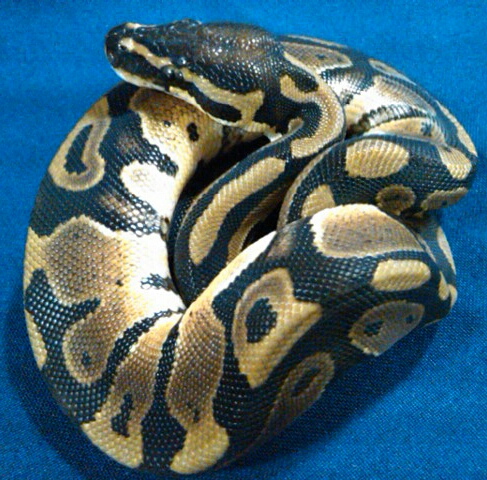
\includegraphics[width=.5\textwidth, height = 62mm]{Normal.jpg}
	\end{figure}
	\begin{figure}[H]
	\centering
	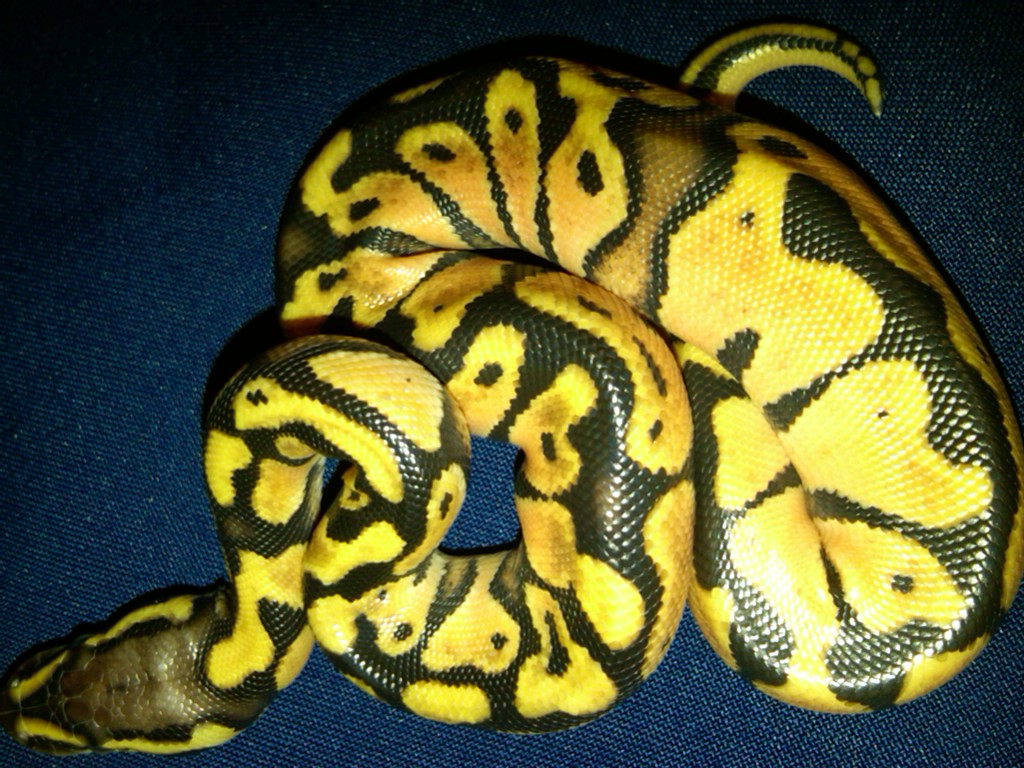
\includegraphics[width=.5\textwidth]{Pastel.jpg}
	\end{figure}
	\end{multicols}
	Note the marked difference that one trait can make in the appearance of the snake. As with dogs, certain traits are valued much higher than others. A Normal costs about \$20, whereas a Pastel costs about \$45, and Ball Pythons with another trait, called Banana, costs about \$200. As one might imagine the `cooler' looking the snake the more it will cost, so breeders seek to make more money by breeding so offspring will express more genes and therefore look `cooler'.\\
	\indent I will not go over the details of snake reproduction here, but there are certain facts that will be used in this paper and the related programs, without which the reader will undoubtedly be lost. Firstly, upon a successful (and sometimes unsuccessful) pairing of a male and female snake a set of eggs, called a clutch, is produced. Secondly, female snakes can breed up to once per breeding season, whereas a male can breed up to five times per breeding season.

	\section*{Theory}
	\indent\indent Initially, one can think of this problem as a portfolio management problem in which the Ball Python breeders are portfolio managers and the snakes are capital goods, and one can imagine that the breeders would like to maximize the present discounted value of profits from their stock of snakes. The preceding method was pioneered in  \cite{jarvis}. Comparative statics for this interpretation have been derived in the preceding paper and \cite{Paarsch}.\\\indent The previous papers assume the animals (cattle) are all homogeneous except in age and there was no improvement in breed over time, which are simply not valid assumptions in the case of snake breeding. The value of each snake in your inventory depends on the genes it expresses, which depends on what its parents were, and there is an overall improvement in your stock over time because of the selective breeding exercise, which can't be handled by the aforementioned model.\\
	\indent One could expect that after a certain point the system will settle into a steady state, and it might be a useful exercise to characterize what the steady state would look like. If the breeder's set of snakes is not homozygous (having two copies of a certain allele) for all the different genes contained in their snakes, then the system will not be in a steady state, since they will try to breed so that their snakes are homozygous for all traits since that makes them more valuable. If their whole stock of snakes is homozygous for all of the same genes except for one snake, then they will either breed the snake that's different to at least one other snake, or they will sell it. If they breed the snake that's different then there will be some snakes in stock that are not homozygous (heterozygous) for all genes, which would continue as selective breeding until all snakes were homozygous for all genes in the stock of snakes. The steady state can't occur unless all snakes have the same genes and are homozygous for them all, at which point the problem changes to be akin to the previous models. However, supposing that all snakes are homozygous for all genes except for a gene which all snakes are heterozygous for, there is some positive probability that in any finite number of periods none of the snakes will be born homozygous for that gene, so a steady state is not guaranteed to be achievable in a finite number of periods.\\
	\indent Suppose instead, that one is interested in how the system behaves before a steady state if one would even occur (as this paper is). As was shown in the previous paragraph, this would be where at least one snake is different from the others, or the snakes are all the same, but not homozygous for all traits. In this world it matters which snake you breed to which, so this becomes a matching  problem: deciding which male to breed to which females. Thinking about a single period yields the problem courtesy of \cite{becker} with a slight tweak:
	\begin{align*}
		\max_{\Pi}&\left\{ \sum_{i\in I}g\left(m_i,f_{\Pi(i)}\right) \right\}
	\end{align*}
	where $I$ is the number of male snakes, $m$ signifies a male snake, $f$ signifies a female snake, $g$ is a profit function, and $\Pi$ is a mapping from the set of males to subsets of 5 or less snakes of the set of females. In this setting the matching problem will result in neither PAM nor NAM (Positive/Negative Assortative Matching) as shown in the simple example below.\\
	\indent Suppose that one has a homozygous Fire male (\$350), a heterozygous Fire female (\$90), and a homozygous Pastel female (\$75). Suppose further that you can only breed one male to one female. The offspring of the Fire Ball Pythons paired together would have an expected value of \$220, whereas with the Fire and Pastel paired together the offspring have an expected value of \$250. This may seem to imply NAM, however if one takes the same females but replaces the male with a heterozygous Pastel (\$45), the expected value of the offspring of Pastel and Fire is \$103.75 and Pastel with Pastel has an expected value of \$60, which contradicts NAM. Now there's a serious problem, if it was PAM or NAM it would be a simple process to choose which snakes to breed to which.\\
	\indent The previous two paragraphs were about a single period decision, which is not really what a snake breeder should be doing. The snake breeder should, ideally, decide what to do this period with an eye to future time periods. Unfortunately, that turns an already difficult problem into an intractable problem, maximizing time discounted profit over an infinite time horizon, i.e.:
	\begin{align*}
		\max_{\Pi_t}&\left\{ \sum_{t=1}^{\infty}\sum_{i\in I_t}g\left(m_i,f_{\Pi_t(i)},t\right)\delta^t \right\}.
	\end{align*}
	\indent So what does one do since true optimality is intractable? The approach this paper uses is find a reasonable rule that does well, where ``well'' is defined as doing better than the rule snake breeders actually follow, and simulate in order to find the changes instilled by a change in the parameters of the system.
	\section*{Data}
	\indent I retrieved the data used for my program from the breeders at a show called Repticon in Tampa.

\bibliography{References}
\nocite{*}
\end{document}